\chapter{Discussion}
\label{chapter-discussion}


%%%%%%%%%%
% Include discussion that the world moves on.

This chapter contains various discussion topics, including: validity of my research and of the analytics tools, where the various analytics tools provide the most value, ethics and legal aspects, abandoned apps, and finally other app stores beyond Google Play.
%TBD whether to include a discussion of:
%%% other analytics tools I've researched during my PhD (e.g. those covered in my probation report)
%%% sweetspots for Crashlytics, Firebase, etc.


Apps are a popular and relevant subset of all software, they run remotely on other people’s equipment where they are the primary owners of the data on their devices, and where the platform and pre-installed platform software determine various aspects of the data collection. The apps and the analytics libraries they use control what data is reported and when. 

At the time of writing neither Apple (iOS) nor Android appear to provide an API for programmers to enable apps to check per-user or per-device preferences for usage and diagnostics information sharing. The lack of such APIs means that each app developer is responsible for deciding whether to ask user's for permission or simply assume their app can collect and send analytics data. 

Listing~\ref{code:androidx_preferences_example} is an example Google provides for Android developers to learn how to use the AndroidX preference library~\footnote{Reproduction permitted as the code sample is released under their~\href{https://developer.android.com/license}{Content License}.}. This example generates a GUI to ask users if they wish to enable message notifications and/or send feedback including reporting technical issues. 

\begin{listing}[H]
\caption{AndroidX preference library example} \label{code:androidx_preferences_example}
\begin{minted}{XML}
<PreferenceScreen
    xmlns:app="http://schemas.android.com/apk/res-auto">

    <SwitchPreferenceCompat
        app:key="notifications"
        app:title="Enable message notifications"/>

    <Preference
        app:key="feedback"
        app:title="Send feedback"
        app:summary="Report technical issues or suggest new features"/>

</PreferenceScreen>
\end{minted}
Source: \url{https://developer.android.com/guide/topics/ui/settings}
\end{listing}


Preferences, permissions, and usage analytics share similarities in terms of considerations such as informed consent, whether the settings are temporary or permanent, and so on.

\section{The WebView component}~\label{section-webview-component}

(something that's used in a vast number of Android apps in my experience, including eBay, GMail~\footnote{\url{https://www.google.com/appsstatus\#hl=en&v=issue&sid=1&iid=aa75515d184a2423be444d676b7ebf45}}), and many others. The BBC development team wrote a detailed and rich blog post~\url{https://www.bbc.co.uk/blogs/internet/entries/3533ce9c-393a-43d8-8f44-0c46214c86aa} on their use of WebViews to host their JavaScript based games for several years. The article includes Wardley Mapping diagrams that position their use of analytics amongst other technologies.

Notes, to be expanded:
\begin{itemize}
    \item \url{https://www.theverge.com/2021/3/22/22345696/google-android-apps-crashing-fix-system-webview} and \url{https://9to5google.com/2021/04/20/android-webview-crash-fix/}
    \item \url{https://play.google.com/store/apps/details?id=com.google.android.webview} 1,000,000,000+ installs, 5,930,222 ratings on \nth{3} June 2021.
    \item \url{https://www.appbrain.com/app/android-system-webview/com.google.android.webview} and possibly discuss the effects of custom WebViews such as from ASUS~\url{https://www.appbrain.com/app/asus-webview/com.asus.webview}
    \item \url{https://www.google.com/appsstatus/ir/fw6156fs1panucr.pdf} Google's explanation of what happened and how they intend to improve matters.
    \item BBC iPlayer app description from \nth{5} April 2021~\citep{bbc_iplayer_app_april_2021_webview_information}.
    \item \url{https://www.bbc.co.uk/news/technology-56496783}
    \item \url{https://www.bbc.com/pidgin/world-56481802}
    \item \url{https://www.bugsnag.com/blog/android-system-webview-causes-apps-to-crash} NB: I don't agree with their claims... App developers should be able to write code that handles at least some exceptions related to WebViews.
\end{itemize}



\subsection{...TBD...}
If we focus on Android apps what are the implications and how relevant are the approaches and results?

\section{On Measurement}
Measurement may begin using rough and approximate measurements and tools, for instance the length of a yard which used to depend on the span of the king's arm~\footnote{One source is:~\url{http://nisltd.co.uk/asp/default.aspx?page=history_of_calibration}}. France, in particular, led to the standardisation of various measurements including the metre~\footnote{\emph{e.g.}~\url{http://www2.culture.gouv.fr/culture/actualites/celebrations/metre.htm} (in French).}.

Software development and testing are still in flux where various people and groups have yet to coalesce or truly agree to common, unambiguous and definitive measurements. Even newer standards, including~\cite{iso29119-1-2013}, which were intended to provide a pragmatic and useful guide to practitioners (\cite{reid2012_iso29119_eurostar}), would only be used by a minority (19\% according to a poll by EuroSTAR Conferences in 2013~\footnote{\url{https://conference.eurostarsoftwaretesting.com/poll-result-will-you-be-using-iso-29119-standards-in-your-testing/})} of an estimated 60 respondents to the poll~\footnote{\url{https://conference.eurostarsoftwaretesting.com/standards-a-case-for-the-defence/}}.

How to measure anything. 

My research into the \emph{use} of mobile analytics tools led into research into the characteristics of several of the actual tools in widespread use by developers of mobile apps. The measurements and assessments of these tools is immature and my work provides a possible starting point to enable these and other analytics tools to be measured and assessed.

\subsection{Inaccuracies in software analytics generally}
Other inaccuracies in various analytics tools provide a backdrop to this research in mobile analytics. For instance, from the domain of ecommerce web sites, a startup, Littledata~\footnote{\href{https://www.littledata.io/}{www.littledata.io/}}, claims 80\% of Shopify merchants are missing at least 20\% of transaction data for those that use Google Analytics to track their transactions and revenues~\citep{littledata2020_google_analytics_doesnt_match_shopify}. The company provides software which claims to provide 100\% accuracy and offer their customers a 30-day free trial to enable a three-way comparison between Google Analytics, Shopify's standard tracker, and their `solution'. Unfortunately for them, the incomplete and misspelt eBook waters-down reduces the confidence in their claims of providing 100\% accuracy. Also, even if two of the systems agree on the transactions and finances these systems are not necessarily correct. Additional evidence, for instance, of all the source events would be needed to cross-verify that what any of the systems report actually matches the inputs.

\section{Debugging in the large}
Debugging in the large is a term presented in Microsoft's research into Windows Error Reporting~\href{glossary-wer}{(WER)} where large scale collection of errors from end-user devices can help developers detect, prioritise, and address various errors that may not appear during development and local testing of the software~\citep{kinshuman2011_debugging_in_the_very_large}. The various mobile analytics services analysed during this research also support debugging in the large (and they suffer from some of the flaws that were reported in WER a decade ago). 

It may be viable to significantly accelerate troubleshooting and reduce the latency by using techniques that were described and applied in a project called CellScope by~\citealp{padmanabha2018_mitigating_the_latency_accuracy_tradeoff_in_moile_data_analytics_systems}. They demonstrated their model was able to make useful and relatively accurate predictions of anomalies in power consumption by mobile apps within one day of the Carat app\footnote{\url{https://play.google.com/store/apps/details?id=edu.berkeley.cs.amplab.carat.android&hl=en_GB&gl=US}}. Unfortunately this Android app was last updated for end users in 2018 and the Carat power recommendation app project no longer appears to be active according to the respective Android\footnote{\url{https://github.com/carat-project/carat-android}, last updated in August 2019} and iOS\footnote{\url{https://github.com/carat-project/carat/}, last updated in February 2018} opensource codebases. Furthermore, the CellScope software does not appear to have been published so future research may need to recreate something similar from scratch.

\section{Threats to Validity}

Let us consider validity from a practical, pragmatic perspective. 
Research by ~\cite{scaffidi2007developing}, states real world developers and users base their decisions on what the paper describes as low-ceremony evidence~\emph{``such as reviews, reputation, advertising claims, qualitative information, or aggregation of group opinion"}. The paper proposes a notation that includes credentials and provenance to help people to systematically adapt their their confidence in software dynamically as new information emerges. Making decisions with imperfect information is also covered in the same paper (~\cite{scaffidi2007developing}) where they discuss \emph{good enough} decision making using \emph{``less-than-perfect information"}. In my industry experience, and in the research described in this thesis, their claims hold true. And in terms of my research I have aimed to assess aspects of the credibility of several analytics tools and provide provenance for the evidence that has been collected during the practical aspects of the research.

Using ratings and reviews to measure quality? Tim Menzies quote on software analytics. 

\subsection{Validity of my research}



\subsection{Validity of the tools being used}

\subsubsection{Validity of platform analytics}

\subsubsection{Validity of Fabric Crashlytics}

\subsubsection{Validity of various mobile apps}

Our simple opensource Android app, Zipternet~\footnote{\url{https://github.com/ISNIT0/zipternet}}, included HTML-based content. In the initial releases the app had a flaw that caused a crash to occur when any external web links were selected in the content~\footnote{See issue 6 on Github for this project:~\href{https://github.com/ISNIT0/zipternet/issues/6}{Fix crash of the app when external URL selected in WebView}.}. This crash occurred consistently whenever any external web link was selected and was detected and reported by Google Play Console's pre-launch report and it was also reported in Android Vitals, albeit less often than when the crash occurred on devices we used for local testing of the app.


In February 2020 the iOS version of the Pocket Code app was enhanced to include a mechanism to cause crashes deterministically~\footnote{See JIRA ticket:~\href{https://jira.catrob.at/browse/CATTY-161}{CATTY-161 - INTERMEDIATE TICKET: Add ``easter egg" for Crashlytics} for the iOS feature.}. This ability to cause crashes deterministically was designed and implemented to determine whether the crashes would be reported correctly in Firebase Crashlytics (they were). The iOS team removed the ``easter egg" immediately after the workshop in Poland~\footnote{See JIRA ticket:~\href{https://jira.catrob.at/browse/CATTY-162}{CATTY-162 - TRAINING TICKET: Remove "easter egg" for Crashlytics}.}. The Android version of Pocket Code already used the older Fabric Crashlytics API and crashes were being reported in the Fabric Crashlytics dashboard.

\subsection{Internal validity}

\subsection{External validity}

\subsection{Ecological validity}
As Wikipedia notes \emph{``Essentially, ecological validity is a commentary on the relative strength of a study's implication(s) for policy, society, culture, etc."} (\cite{wikipedia_ecological_validity}).

One of the aims of my research is to determine whether it is applicable for and relevant to real-world developers of mobile apps. 

Working with non-profit opensource projects, where the teams are generally willing to make their practices and results public, helps with being able to obtain information and publish the results. However, as many research projects discover, what might work for opensource projects -- while important and interesting to the research community -- might not matter much to the industry of professional and commercial development teams. 

Opensource apps are a tiny proportion of mobile apps available to users, so another level of learning and validation could be achieved through the insights of these professional and commercial development teams. Surveys tend to have poor response rates and lack the depth or richness I was seeking therefore I chose to engage at a deeper level as a fellow developer interviewing developers of several apps. Of course we would need the permission of their organisations, and some shared examples of their tools, their practices and their results of applying analytics well, and even times when they hadn't.

I have been fortunate to receive external confirmation from various external sources that the research is of interest and appears to have some validity. These include: validation from the Google engineering team responsible for Android Vitals and Google Play Console. It also includes validation from developers of mature opensource and commercial Android applications. 

One of the challenges in this research has been to balance internal, external and ecological validity, a challenge others have faced in their research in other areas including educational software (~\cite{ransdell1993educational_software_evaluation_research_validities}) where they realised there are multiple factors that influence the outcomes and results of their experiments and research. Similarly, real-world development of mobile apps, and changes in the stability of their apps depend on multiple factors. And from a research perspective, it was, and is, impractical to observe or measure everything that might contribute to the changes in stability, etc. What does appear to be clear are two related factors:

\begin{enumerate}
    \item When developers pay attention to flaws reported in analytics tools they are able to effect improvements to the app which significantly reduce the failure rate and improve the stability of the apps for end users.
    \item Developers will release updates that unintentionally and or exacerbate the failure rate, despite their best intentions. They need to pay ongoing attention to the reported failures if they wish to maintain or decrease the measured stability of their apps as both their app and the ecosystems evolve~\footnote{Ecosystems evolve as new devices, operating system releases, networks, updates to libraries, and to other related apps and components (such as the Google \href{ection-webview-component}{WebView component}), etc. change.}.
\end{enumerate}

\subsubsection{Validity from the Google Engineering Team}



\subsubsection{Other validation}
In email discussions of my research in 2020 one of the leading authors in the field, \href{https://scholar.google.com/citations?user=zuUsFkgAAAAJ&hl=en&oi=sra}{Li Li}, confirmed the novelty, importance and relevance of my research.



\section{Do the concepts scale?}
This research is limited to apps available in Google Play for practical reasons. Here we consider whether the approach could scale beyond Google Play for Android apps, and later whether the approach could work for other platforms.

\subsection{Beyond Google Play?}
Other Android app stores are available, particularly in China as~\citep{wang2018_beyond_google_play} describes. Of the Chinese app stores, in 2018 only 2 (Tencent Myapp, and 360 Market) provided a quality rating. Their work indicates that at least some app stores are not likely to provide stability analytics similar, or equivalent, to those Google provides in Google Play Console and Android Vitals. Developers, therefore, would need to implement any analytics into their app rather than rely on the app store. Two more recent app stores are discussed next: Huawei and Amazon.

\textbf{Huawei}: 
Huawei needed a comprehensive alternative to the Google Android ecosystem, driven by the ramifications of the ongoing ban in the USA~\citep{androidauthority2021_the_huawei_ban}. 
% And https://www.cnet.com/news/huawei-ban-timeline-chinese-company-android-rival-coming-phones-tablets/
They have been ramping up their app store~\citep{androidauthority2021_huawei_app_gallery}, known as \href{https://appgallery.huawei.com/}{HUAWEI App Gallery}. According to~\citep{vodafone2021_huawei_appgallery}, it had over 180 billion downloads in the past year - which would infer lots of usage of those downloaded apps and very likely lots of crashes! 
%
In 2020, Huawei announced \emph{``HUAWEI is one of the world's top three application store"} [sic]~\citep{huawei2020_press_release_on_hms_ecosystem}, serving 600 million Huawei device users. In March 2021, Huawei stated they have over 2.7 million developers outside the Chinese Mainland~\citep{}. 
Huawei are rolling out their Android operating system HarmonyOS to a wide range of their existing devices~\footnote{\url{https://www.huaweicentral.com/huawei-harmonyos-upgrade-plan-devices-and-rollout-time-list/}} which may accelerate the growth of activity in their app ecosystem. In short, they have a large and growing ecosystem with lots of apps and users of those apps.

Huawei provide an optional Analytics SDK for developers~\citep{huawei_analyticskit}; in turn it provides a crash and error reporting SDK together with a Codelab~\citep{huawei_crashservice_codelab} and examples~\citep{huawei_crashservice_github_examples}. They encourage developers to test the crash reporting and their API includes facilities to enable and disable crash collection, to generate a test crash, to record Exceptions, and to report custom events~\citep{huawei_ag_connect_crash}. 
Their crash reporting appears to be integrated in an online console for developers~\footnote{\url{https://developer.huawei.com/consumer/en/console}~\citep{huawei_introduction_to_appgallery_connect_crash_service}}. 

They also provide a programmatic data export service~\citep{huawei_analyticskit_dataexport_codelab}. According to one of their developer-oriented articles~\citep{huawei_introduction_to_appgallery_connect_crash_service}, \emph{``The crash rate of a problem is greater than the threshold 1\%"}~\citep{huawei_introduction_to_appgallery_connect_crash_service}, which is similar to Google's bad behavior threshold of 1.09\%. In their AppGallery Connect Service whitepaper they mention crashes and ANRs in an image titled \emph{``Analysis: Driving Operations Decision-Making with Data"}, however the whitepaper did not provide any more details on how the information would be collected or provided~\citep{huawei_appgallery_connect_service_whitepaper}. 

\begin{comment}
\begin{itemize}
    \item How to enable the Analytics service~\url{https://developer.huawei.com/consumer/en/doc/development/HMSCore-Guides-V5/service-enabling-0000001050745155-V5} and see \url{https://developer.huawei.com/consumer/en/codelabsPortal/carddetails/HMSAnalyticsKit}. There's also a codelab for enabling analytics in Kotlin~\url{https://developer.huawei.com/consumer/en/codelabsPortal/carddetails/HMSAnalyticsKit-Kotlin}. There's also the article on Medium~\citep{huawei2020_appgallery_connect_crash_service_article_on_medium} and the associated source code on GitHub~\url{https://github.com/SerkanMUTLU/Huawei-AppGallery-Crash-Service}.
    \item How the Crash Service works \url{https://developer.huawei.com/consumer/en/doc/development/AppGallery-connect-Guides/agc-crash-introduction-0000001055732708}. Three steps: 1) integrate the SDKs, 2) test the crash service, and 3) analyse a crash. 
    \item Their Android Sample Code is available \url{https://developer.huawei.com/consumer/en/doc/development/HMSCore-Examples/android-sample-code-0000001050745043}
    \item Pre-release Check for their Analytics SDK \url{https://developer.huawei.com/consumer/en/doc/development/HMSCore-Guides-V5/android-pre-release-check-0000001050420841-V5}, which includes a spreadsheet (which I've downloaded) that covers basic sanity testing.
    \item Lots of clear articles (still lacking in various details) that help to understand how their analytics SDK behaves and how that behaviour can be modified (and checked) by developers. For example~\citep{huawei_accessing_analytics_kit}.
    \item Online training videos on their Analytics software \url{https://developer.huawei.com/consumer/en/training/detail/101582991973534154}
    \item Cloud Testing articles \href{https://forums.developer.huawei.com/forumPortal/en/topic/0201271583209350068}{Part 1} and \href{}{Part 2}. And a more structured article~\url{https://developer.huawei.com/consumer/en/doc/development/AppGallery-connect-Guides/agc-cloudtest-introduction-0000001083002880}.
    \item Developer reports he cannot see crashes for the productFlavor that should use the Huawei crash reporting~\url{https://stackoverflow.com/questions/64800108/can-not-see-crashes-for-android-on-appgallery-connect}. It's not clear whether a) the library needs to be instantiated by the application at runtime, b) if there'll be conflicts between the Huawei and Google Firebase crashlytics libraries and/or instantiation.
    \item \url{https://developer.huawei.com/consumer/en/appgallery/} marketing to the developers.
    \item \url{https://developer.huawei.com/consumer/en/codelabsPortal/index} HUAWEI Codelabs.
    \item \url{https://stackoverflow.com/questions/tagged/huawei-mobile-services} Active support from Huawei for developers.
    \item \url{https://stackoverflow.com/questions/67885601/react-native-app-crashes-while-launching-after-implementing-hmscore} Interesting answer from Shirley who works for Huawei I believe about how their support HMS Core on non-Huawei devices \url{https://stackoverflow.com/a/67886284/340175} - Details saved in my references in the HUAWEI folder.
    \item App Rollbacks \textit{are} supported! \url{https://developer.huawei.com/consumer/en/doc/distribution/app/agc-help-rollback-0000001146534647}
    \item Developers can provide messages in the app store for their users \url{https://developer.huawei.com/consumer/en/doc/distribution/app/agc-help-developers-message-0000001146438657}
    \item \emph{Intermediate: Easy fix of application crash using Huawei Crash Service and Remote Configuration}~\url{https://forums.developer.huawei.com/forumPortal/en/topic/0202581794223780039}
\end{itemize}
\end{comment}

Huawei have published a ``success story" of how Doodle Draw used Huawei's crash service to detect and then resolve an \emph{``unexpected exit problem"} on the day they started using the crash service. The crash rate of the app was then \emph{``decreased from 1\% to 0.06\%, greatly improving the app quality"}~\citep{huawei_agc_success_stories}. It is slightly ironical their article discusses ``success stories" yet there is only one success story, more have been requested.

Key differences between their provision and that provided by Google include the lack of integrated platform (device-level) analytics from the Operating System, the need for developers to integrate a full Analytics SDK in order to then use the crash and error reporting SDK. They do not mention of the equivalent of Android Vitals. In terms of pre-release checks and testing, they provide various elements that offer similar capabilities to the pre-packaged pre-launch reports that Google Play Console provides. For example, they have an Integration Check~\citep{huawei_appgallery_integration_check} which appears to perform various forms of static analysis and Cloud Testing~\citep{huawei_appgallery_cloud_testing} that in turn includes similar automated testing capabilities. 

As Huawei develops HarmonyOS and their app store, potentially platform-level analytics could be added and made available by Huawei in future.

\textbf{Amazon app store}: 
Another major app store for Android apps is the \href{https://developer.amazon.com/apps-and-games}{Amazon appstore}, which includes `millions of devices in over 236 countries and territories'. They provide an \href{https://developer.amazon.com/settings/console/home}{amazon developer console} which offers a subset of the Google Play Console's features together with some Amazon specific product and service offerings. 

Many, but not all, of Google Firebase Android SDKs are able to be used beyond Google Play. The other SDKs require Google Play services which is part of the Google Android platform. And uniquely, firebase-analytics states `\emph{automatic insights such as demographics are only available on devices with Google Play services.}'~\citep{firebasesupport2020_dependencies_of_firebase_sdks_on_google_play_services}. 


\textbf{Could the techniques improve reliability beyond Google Play?} 
These brief introductions into Huawei's and Amazon's, global app store ecosystems indicate there provide sufficient developer-oriented tools and services for developers to be able to measure reliability of their Android-like apps were they distributed in these app stores, and to be able to use the analytics offered by these providers (and potentially other analytics providers, for instance Countly claims their Android SDK should work on HarmonyOS~\citep{countly_which_operating_systems_are_supported}) to identify reliability issues and potentially address them. Neither of these ecosystems currently provide the richness of the Google Play Console or Android Vitals, they could choose to do so in future and the underlying Android based operating systems could gather similar data, at least from a technical perspective.

\subsection{Beyond Android?}

Apple also provides a platform and an app store (called the `App Store'). 

For iOS Apple describes how developers can collect crash reports from TestFlight and from the App Store. In the same article they describe how users can locate and email crash reports and email them to the app's developer, for instance if the developer does not have them. They do not explain how the developer or user reach each other to communicate about the crash or the contact details~\footnote{\href{https://developer.apple.com/documentation/xcode/diagnosing_issues_using_crash_reports_and_device_logs/acquiring_crash_reports_and_diagnostic_logs}{Acquiring Crash Reports and Diagnostic Logs}.}. 
%
Apple also provide practical advice on how to diagnose issues using crash reports, memory inefficiencies using `jetsam event reports' and problems using `device console logs'~\footnote{See Xcode documentation:~\href{https://developer.apple.com/documentation/xcode/diagnosing_issues_using_crash_reports_and_device_logs}{Diagnosing Issues Using Crash Reports and Device Logs}.}. 
% 
From various online discussions~\footnote{Examples of discussions on iOS crash logs include:~\href{https://stackoverflow.com/questions/10145665/crash-reports-from-app-on-app-store}{Crash reports from app on App Store}, and the poorly titled forum post ~\href{https://developer.apple.com/forums/thread/30934}{App Analytics Crashes}.} 
% See also https://stackoverflow.com/questions/50709109/ios-app-store-get-crash-reports
The iOS analytics include some of the reporting and analysis provided by Google in the Google Play Store tools, for instance~\emph{``...how crashes break down across OS versions and different devices"}~\cite{apple2020_how_to_review_your_apps_crash_logs}. Their reports currently lack some of the more sophisticated reporting that Google Play and Android Vitals provide. Nonetheless, sufficient raw elements are available to developers to enable them to discover crashes and memory issues from end users in order to address these. Apple also launched Feedback Assistant in 2019 with the aim of enabling people to submit effective bug reports using either an app or a website~\cite{appledeveloper2020_bug_reporting_feedback_assistant_for_developers}. Authorised members of the app's development team can access and review the feedback reports using similar tools~\cite{appledeveloper2020_bug_reporting_feedback_assistant_for_developers}.



\subsection{Quis custodiet ipsos custodes?}
\url{https://en.wikipedia.org/wiki/Quis_custodiet_ipsos_custodes\%3F}
Who watches the watchers? The app store is all powerful, promoting one app, demoting or even blocking another. What it reports is expected to be taken on trust. And who has time or resources to check or verify the veracity of what is being reported and to whom? As the Editorial Board of the Financial Times proposed three rules to build trust in the use of automated algorithms in decision making~\emph{``algorithms that companies and governments deploy in sensitive areas such as healthcare, education, policing, justice and workplace monitoring should be subject to audit and comprehension by outside experts."}\citep{ft2021_building_trust_in_ai_systems_is_essential}. Given the revenues, powers and business implications of the major app stores, I believe they should also be subject to audit and comprehension by outside experts.

To the credit of several providers of analytics SDKs, including Crashlytics and Huawei's crash reporting SDK, they provide mechanisms to test their crash reporting service. However, these tests do not necessarily mean the analytics are completely accurate, reliable, and scalable. For example, in an online tutorial, a developer at Huawei explained~\emph{``Note : If an error is occurred in try catch block, Crash service won’t catch it. Crash Service just catches critical error that is stopped app"}~\citep{huawei2020_appgallery_connect_crash_service_article_on_medium}. Conversely, Google Android collects usage statistics from small percentages of users from WebView components incorporated into Android apps including crash reports~\footnote{An example of WebView crash reports for specific Samsung device models is discussed on Stack Overflow~\citep{ebling2018_so_s9_specific_webview_device_crash_report}}. Google discusses user privacy implications in these crash reports~\citep{android_webview_privacy}.

Also, as Huawei acknowledged in the version history for their Android SDK their SDK previously caused some crashes (in versions 1.5.0.300, for instance) and needed improvements in the crash rate (in version 1.5.2.300) accuracy~\citep{huawei_android_crashservice_sdk_version_change_history}. Similar issues may well exist in other Analytics SDK and related services. 

It's encouraging to see Huawei's honesty which increases their credibility in this area. Even better would be for all the analytics providers to release the source code and the measurement techniques they use so both of these can be independently checked and verified.


\subsection{Necessary? Sufficient?}
Freezes and crashes may adversely impact a user's perspective, Google may limit the visibility of apps that score poorly in terms of 'stability' as I will cover later in my thesis. However, are performant applications sufficient to thrive? There may be other barriers, or hurdles, developers need to overcome such as providing software that is attractive, serves whatever the user wants to do, and is intuitive.

Research published by Microsoft on Windows Error Reporting (WER) states~\emph{``WER augments, but does not replace, other methods for improving software quality."}~\citep{kinshuman2009_debugging_in_the_very_large, kinshuman2011_debugging_in_the_very_large}. Similarly, using mobile analytics to find and prioritise failures to address augments rather than replaces other methods for improving software quality. For failures that are able to be detected and reported using mobile analytics - relying solely on using mobile analytics to detect and address them may overwhelm developers in fix, patch and release cycles rather than other improvements to the app. Furthermore users of these failing apps may simply stop using it, reject it, and the developers who provide the app~\citep{dimensionalresearch2015_mobile_app_use_and_abandonment}. Other quality issues that mobile analytics does not capture, need to be addressed using other techniques and tools.

In 2019 Menzies in his paper \emph{``Take Control: On the Unreasonable Effectiveness of Software Analytics"}~\cite{menzies2019take} indicates that a small number of predictable software analytics variables can be used to predict software qualities for projects. 

\emph{``Specifically, the number of variables required to make predictions about SE projects is remarkably small which means that (a) most of the things we think might affect software quality have little impact in practice; (b) controlling just a few key variables can be enough to improve software quality."}


\section{Trade-offs of: ``Fail Early"?}
Fail Early has been argued as a helpful policy in various contexts MUST-DO expand and provide examples. Fail Fast mentioned in~\citep{gray1986_why_do_computers_stop_and_what_can_be_done_about_it} but not explained or discussed. Make bugs easy [easier] to find~\citep{shore2004_fail_fast_software_debugging}.

The benefits of applying a fail fast approach are described in~\citep{shore2004_fail_fast_software_debugging} with the aim of immediate and visible failure. For rare failures and those the developer cannot easily track down, this approach may help the developer learn about causes of the failures (for instance by raising an explicit exception in the program) where the failure is reported by mobile analytics. For platform level analytics, these fail fast failures would result in crash clusters reported by the analytics. However, Android Vitals does not currently include the message portion of exceptions. The examples in~\citep{shore2004_fail_fast_software_debugging} make extensive use of the messages for communications, so when developers rely on platform-level analytics they may need to consider ways to augment the communications of failures (such as incorporating a crash reporting library or service into their app)~\footnote{We did explore an alternative approach, where the application code added meta-information as an entry in the stack trace as a proof-of-concept, the implementation is available online at~\href{https://github.com/ISNIT0/AndroidCrashDummy/blob/cfa7f0817c436d7e657741e0a5d9a76644e5a898/app/src/main/java/com/example/user/androidtestapp/MainActivity.java\#L28-L50}{AndroidCrashDummy MainActivity.java\#L28-L50}.  However, we decided not to release an app in Google Play with this capability at the time.}. For in-app analytics the developer has the option to report the error using the respective API. An example of reporting an error with additional parameters is shown in Listing~\ref{listing:microsoft-app-center-handled-exception}~\footnote{The Microsoft App Center documentation is released under a Creative Commons Attribution 4.0 International Public License~\href{https://github.com/MicrosoftDocs/appcenter-docs/blob/live/LICENSE}{App Center Docs LICENSE}.}.

\begin{listing}
\begin{minted}[
    gobble=4,
    frame=single,
    fontsize=\tiny,
    breaklines=true
  ]{java}
try {
    // your code goes here.
} catch (Exception exception) {
    Map<String, String> properties = new HashMap<String, String>() {{
        put("Category", "Music");
        put("Wifi", "On");
    }};
    Crashes.trackError(exception, properties, null);
}
\end{minted}
\caption[Microsoft AppCenter: example of reporting a crash in Android]{Example of reporting a crash in Android.  Source~\href{https://docs.microsoft.com/en-us/appcenter/sdk/crashes/android}{ Microsoft App Center documentation}}
\label{listing:microsoft-app-center-handled-exception}
\end{listing}


When developers do not write exception handlers for parts of their code, unhandled exceptions cause the app to crash when they occur. The user may be annoyed by this behaviour if the crash visibly~\footnote{Here visibility refers to the user noticing the crash and being aware of the crash adversely impacting their experience.}  affects their use of the app. The aphorism, \emph{`every cloud has a silver lining'}, may yet hold true in these circumstances provided developers become aware of the crash and choose to address it suitably, as these crashes are detected by various mobile analytics tools and platforms and then reported to the development team.

In contrast a lukewarm, and sometimes expedient approach, is where developers add minimalist \texttt{try\{\}...catch\{\}} handlers to wrap the code that may throw an exception. These exceptions are no longer `unhandled' however nor are they adequately handled in terms of the application providing error management, or attempts to recover from the error, or informing the user of a problem that's occurred, and so on. MUST-DO provide some code snippet examples and analysis of the prevalence of the use of this approach.

To add to the complexities, app stores are seldom disinterested observers. If the measured crash rate increases beyond what they deem an acceptable threshold (1\% for Huawei %~\citep{huawei_introduction_to_appgallery_connect_crash_service}
, 1.09\% for Google Play's bad behavior threshold) they may reduce the visibility of the app in the app store and/or otherwise mark it down. Therefore developers need to be mindful of their strategy to crashes and crash reporting and aim to keep the overall failure rate of their app well below any bad behaviour threshold.

Using software libraries can also add to the complexities; and some have sophisticated error handling strategies which include expectations on how developers will write their code to use that library adequately. RxJava is a very popular library for Android apps. That library explicitly changed their error handling strategy in version 2.0 and require developers to abide by their requirements for error handling~\footnote{\url{https://github.com/ReactiveX/RxJava/wiki/What's-different-in-2.0\#error-handling}}. In version 2.0~\emph{``RxJava defaults to printing the Throwable's stacktrace to the console and calls the current thread's uncaught exception handler."}. The wiki page goes on to say~\emph{``Unfortunately, RxJava can't tell which of these out-of-lifecycle, undeliverable exceptions should or shouldn't crash your app."} So developers who use this library may end up with their app terminating abruptly where the reported crash rate also increases as a result.

% MUST-DO subject to approval or a suitable alternative example: add the OkHttpv3 example from the large case study in the relevant section, then discuss the example here.

\textbf{Measuring reliability}: 
Failure rates include: unhandled exceptions, ANRs, and errors. Errors include: handled exceptions that are recovered from, caught exceptions, logic errors, calculation and content errors, and many others. 

Even \textit{if} an app catches and 'handles' every exception it may not be truly reliable \textit{i.e.} there may be various errors that occur that do not lead to a runtime exception or an ANR. As such, the measured failure rate - assuming it is accurate or undercounting - is the lower bound of the true error rate.

\section{Mitigation techniques}
Summary: \textit{Reduce the incidence, reduce the severity, prevent the trigger, fix if and when practical given the many constraints the team, and the individuals,  are operate under.}

\subsection{Approaches to reducing failure rate}
There are many approaches to reducing the measured failure rate. The `logical' one is to fix whatever the cause is, or at least write code that handles causes robustly, reliably and in ways that serve the user well. And if this is easy and practical many developers and projects will adopt this approach. However like many things that involve people and their motivations they may choose other approaches for various reasons, such as:

\begin{itemize}
    \item Information gathering: where the cause of a failure is not known and not understood, programmers may add code to collect and report additional information to enable them to learn enough about the context of the failure in order to address it once they have learned enough to do so.
    \item Error masking: for instance, catching an exception so it does not get reported or counted.
    \item Error avoiding: change the flow of control of the code so the unreliable path is avoided where practical.
    \item Reduce the incidence: in a similar way to back-off retry algorithms used elsewhere in software~\footnote{For example, back-off algorithms were designed into Ethernet retransmissions, in logins after previous logins failed, and used in GMail for retrying failed connections, \emph{etc.}} apps can be coded to reduce the frequency of failures. 
    %%%% See also https://github.com/OWASP/owasp-masvs/blob/master/Document/0x09-V4-Authentication_and_Session_Management_Requirements.md
    % https://mobile-security.gitbook.io/mobile-security-testing-guide/general-mobile-app-testing-guide/0x04e-testing-authentication-and-session-management
    \item Functional amputation: generally that of failing code deemed so flawed it is not worth trying to correct. Post amputation a replacement may be provided, perhaps from another source and either used instead or grafted into the current project (for instance using an external software library). The replacement of the custom downloader in Kiwix Android is one example where this approach was used.
    \item Blocking: Prevent users from using the app on devices where severe problems occur, \emph{``... exclude those devices until a fix is available."} is one approach recommended in Google's Android Vitals Best Practices~\cite{android_vitals_best_practices}.
\end{itemize}

Note: a reviewer of an earlier version of the above list argued they were merely bad software development practices - perhaps. And yet, empirically they are practiced to varying degrees and may mitigate against high failure rates when it is impractical to fix a cause quickly, completely, and efficaciously.

Fixing bugs may be considered a chore~\citep{scrumdictionary_chore} by many, and there are discussions in the context of Agile software development practices whether work on bugs should be allocated story points at all~\emph{etc.}~\citep{se2012_story_points_for_bug_fixing_tasks_in_scrum} where one respondent was adamant that they should not, otherwise developers would be earning points for poor quality work~\footnote{\url{https://softwareengineering.stackexchange.com/a/162166/93935}}; furthermore the tester is blamed for not finding the bugs (as if that were a) practical or b) appropriate). In response to seeing three crash clusters for their app a project manager responded~\emph{``I don’t know how broad these categories are, but my understanding is that fixing bugs isn’t the sexiest thing to do in life. What if we could free up some budget and hire a team to do the boring work?"}~\footnote{From an unpublished email discussion on addressing crash clusters.}  Those who fix bugs rather than work on features may be perceived as adding less value to a project or team, hence the seemingly illogical `bad' practices may actually be logical in terms of game theory. Interesting research is emerging in applying game theories to software development~\citep{GAVIDIACALDERON2021_game_theoretic_analysis_of_software_development_practices} and may help provide insights into how sources of crashes and other failures are addressed in practice and lead to improvements to reliability of mobile apps through applying game theories.

\subsection{Disproportionate returns}
The failure footprint~\footnote{A first approximation of a suitable measure of a failure footprint is multiplying the frequency by the number of affected users. Projects may choose to develop their own algorithm if this is not sufficient for their context and needs.} varies, as does the effort needed to address specific failures. As noted in the Kiwix case study, fixing two of the top three most frequent crashes reduced the overall crash rate by around a third. Neither of the fixes were complicated. This does not hold true for all failures, some have a tiny footprint, for instance one developer (for the opensource SmartNavi Android app)
mentioned they had seen a few sporadic crashes on phone models they had no access to and decided it would be futile to try and address these crashes in the circumstances. Similarly, the lead developer for the GTAF Android apps explained the developers consider the ease of fixing crashes before tackling them. 

Developers therefore can obtain higher returns in terms of improvements in measured quality if they choose to fix causes that lead to the most frequent failures where the time-to-repair is small. A company analysed 1 billion java errors recorded in logs and determined that fixing the top ten most frequent errors would reduce the crash rate by 97.3\%~\citep{overops2021_what_causes_97pct_of_1billion_java_logged_errors}. Their article does not explore how practical it would be to address those ten errors. This research, on using mobile analytics, has not yet encountered any mobile apps where so few crashes are the cause of so many errors, nonetheless both the research and this example from industry illustrate the value in fixing the worst offenders provided the bugs are tractable and easy to fix within the timescales available to the developers. Furthermore, mobile analytics done well helps keep the signal to noise ratio high in terms of aggregating and reporting on patterns of failures.

\section{Android Vitals}
\subsection{Which apps can Android Vitals help?}
As Google only provides various reports in Android Vitals once they decide enough data exists to preserve the privacy of end users Android Vitals provides little for developers of less popular apps. 

Based on very rough approximations combining my case studies with AppBrain's download statistics to 19th June 2019, shown in figure \ref{fig:appbrain_download_statistics_jun_2019}\cite{appbrain_download_statistics_june_2019}, of the total populations of app developers:
\begin{itemize}
    \item 3\% to 4\% (those with 100,000 to 500,000 total downloads) will get limited value as at least one report will be provided.
    \item < 1\% (those with 500,000 to 1,000,000 total downloads) will get some value as many of the reports will be provided, but not all.
    \item 1\% (those with > 1,000,000 total downloads) will get extensive value as most/all the reports will be provided.
\end{itemize}

\begin{figure}[!htbp]
    \centering
    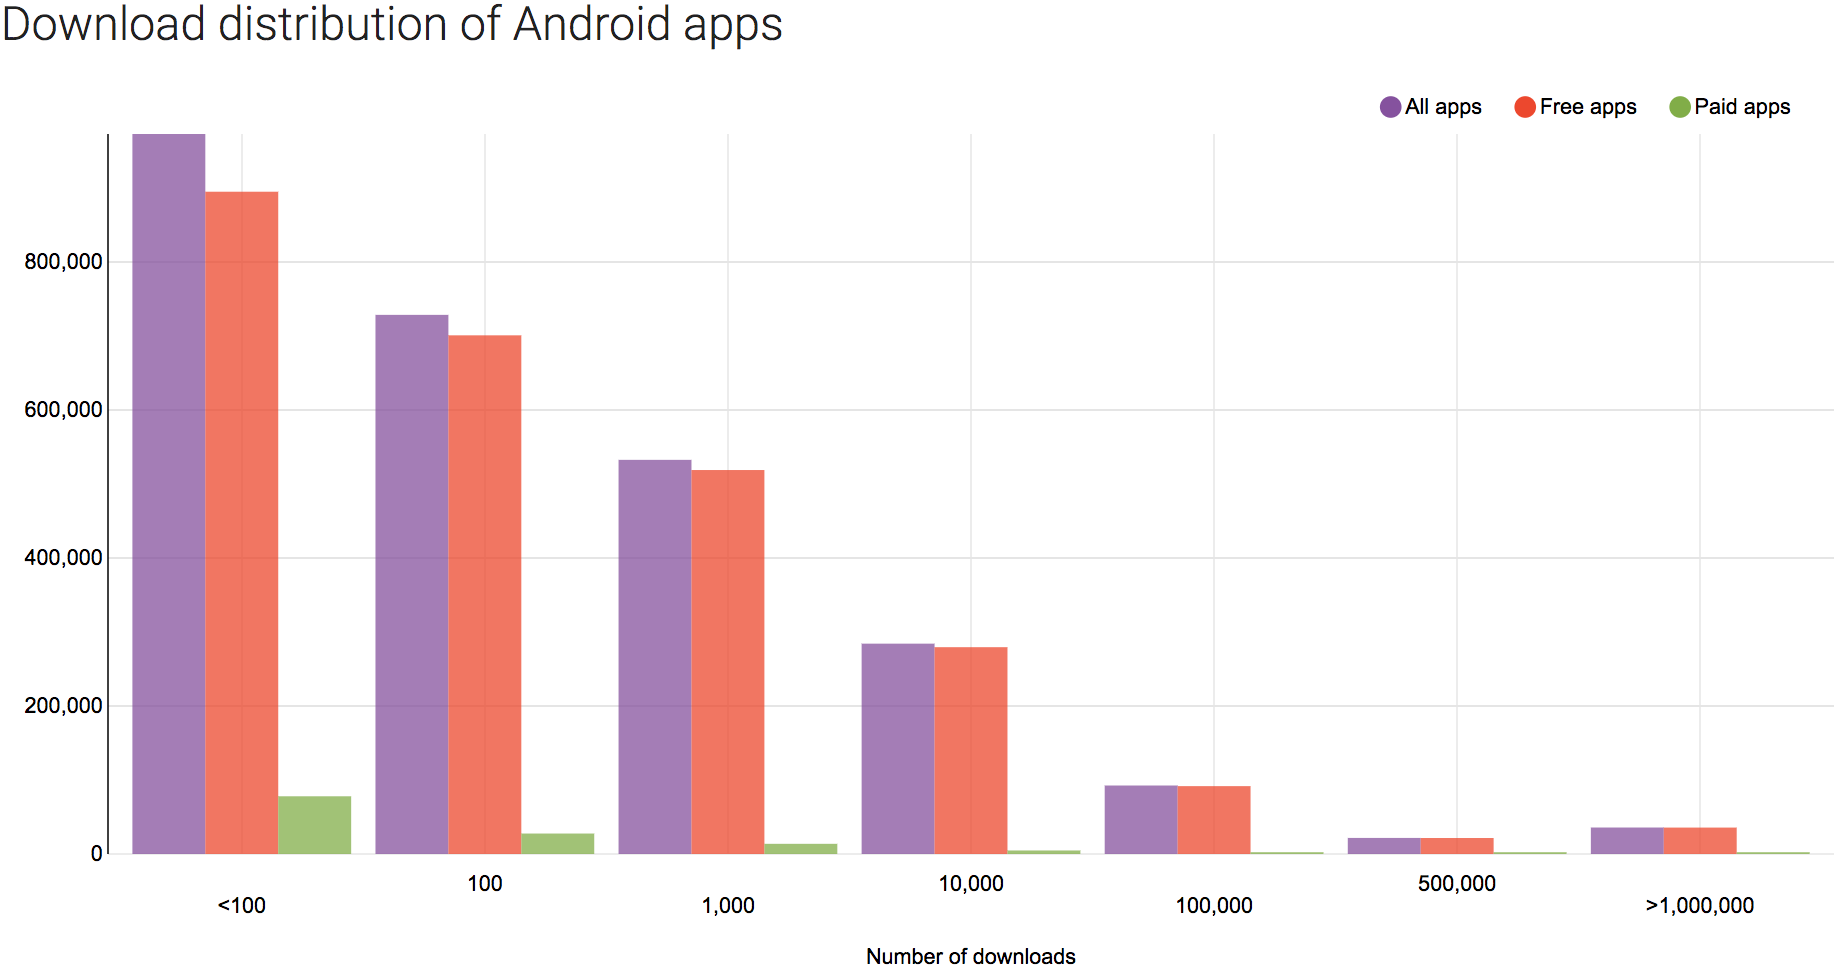
\includegraphics[width=\textwidth, keepaspectratio]{images/appbrain/AppBrain_Download_Statistics_20-Jun-2019.png}
    \caption{AppBrain: Download distribution of Android apps (June 2019)}
    \label{fig:appbrain_download_statistics_jun_2019}
\end{figure}

\subsection{Limitations in using Android Vitals for Observability}
Observability provides two key benefits according to~\citealp{lightstephq2021_observability_will_never_replace_monitoring}: 1) monitor key signals, and 2) understand changes in a system. Mobile analytics facilitates observability of mobile apps, and in particular Android Vitals facilitates the observation of app startup times, performance, ANRs and crashes that occur when an app starts-up. However the inability of storing and analysing the data over time in Android Vitals (beyond the standard reports and recent failure details) limits the ability to observe and analyse stats and/or failures over time.



\subsection{Who gets sufficient usage to see more detailed reports?}
Our limited insight into Android Vitals already indicates that reports are only provided when there is sufficient data collected to 'prime the pump'. It may be possible to estimate how many apps of those in Google Play Store are likely to have enough volumes of usage data. Google makes various recommendations for developers on how to apply the results Android Vitals reports \url{https://developer.android.com/distribute/best-practices/develop/android-vitals} however the developers can't do much until Android Vitals actually shows them the data. For apps with less than about 50k active installs \textit{("Installs on Active Devices (devices online in the past 30 days with this app installed)}." according to Google Play Console's tool tip). These counts are around 20\% to 30\% of the total install count for various apps used in our research \textit{e.g.} the active installs would be around 20k for an app that shows at having 100,000+ [total] installs to end users in Google Play.

Data provided by AppBrain~\cite{appbrain_download_statistics_june_2019} was used to estimate the populations of apps that are not likely to generate enough data to see various reports in Android Vitals.
% wikimedes 5373 active installs - Crash rate by app version only (not device or Android version).
% wikimedzh 3769 active installs - no Android Vitals reports
% wikimedfa 2807 active installs - no Android Vitals reports
% 
Based on Android Vitals reports for Kiwix custom apps we infer that few apps with less than 20,000 total installs will have any detailed reports; WikiMed in Spanish has 5,373 active installs and has one report, for crash rate by app version. None of the other reports are available for this app. The threshold for when there is enough data for Google to provide a report depends on various factors, so the total installs is a proxy measurement and imperfect. Therefore Android Vitals is unlikely to offer much value for developers of (973,381 + 730,419 + 553,261 + 284,634) apps i.e. 2,541,695 apps in Google Play. For the next 92,678 the value of Android Vitals might increase somewhat, depending on how their app behaves and their user-base (e.g. are they on a few Android versions or spread across a spectrum - the larger the spread the less likely the reports will have data). And so on. By my admittedly limited view into the overall data set, Android Vitals is best placed to help the developers of the top (21,728 + 35,854) 57,582 apps, approximately 2\% to 3\% of the total population (2,691,955 apps). These apps (according to AppBrain's data on library use) are also more likely to use Firebase, Crashlytics, etc. so also have some of the run-time data available from these sources in addition to Android Vitals.

My work is to investigate two broad sources of data - data collected by the operating system (here effectively what appears in Android Vitals) and data collected using in-app libraries, particularly mobile analytics, it could include heatmapping (e.g. Appsee, found in over 790 Android apps with over 375 million downloads~\cite{appbrain_appsee}), crash handlers, etc. to provide feedback to measure how well the development team did in terms of testing and code quality. What they learn could also be useful to help them improve how they develop and test their apps in future, particularly with the greater detail mobile analytics (particularly Firebase) can provide the team.

\subsection{All that glitters is not gold}
Android Vitals sometimes reports excessive network usage running in the background while the device is running on battery, as shown in figure \ref{fig:android_vitals_excessive_network_usage}. As the Kiwix app is designed to enable users to download sometimes extremely large files, and to do so in the background, this warning is to be expected and not a bug - it's a feature. So, not everything that Android Vitals flags necessarily needs to be acted on. % c.f. EduVPN's behaviour. 

% Isabel mentions why devs don't use paper: https://scholar.google.com/scholar?hl=en&as_sdt=0%2C5&q=emerson+murphy+hill+static+analysis&btnG=

\begin{figure}[!htbp]
    \centering
    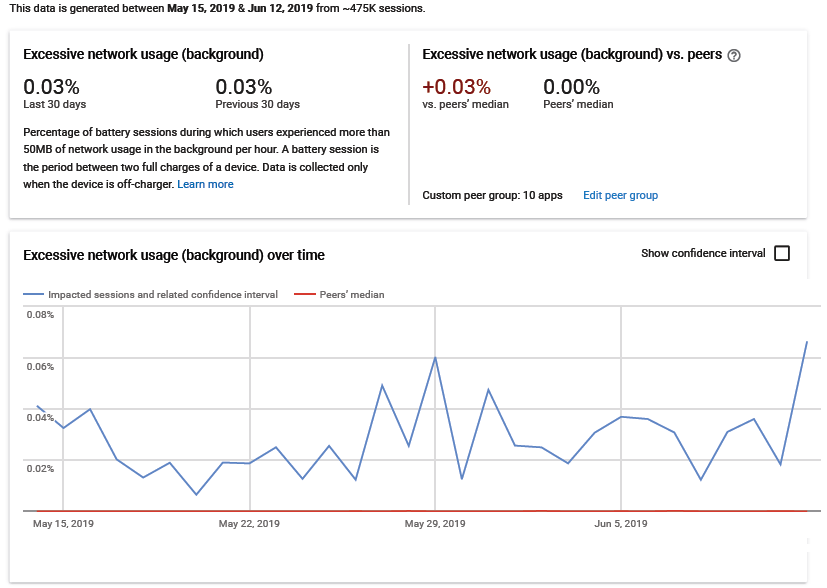
\includegraphics[width=\textwidth, keepaspectratio]{images/android-vitals-screenshots/Excessive_network_usage_by_kiwix_15_jun_2019.png}
    \caption{Excessive background network usage on battery}
    \label{fig:android_vitals_excessive_network_usage}
\end{figure}

\section{Ethics of incorporating mobile analytics}
Tradeoffs; comparing other approaches which may have similar effect with less/no tracking.

Our work exists within a wider context and in society, and the choices we make when we design and implement software and related systems may affect the lives of many people. This applies for those working with mobile apps. Recent investigations into 5000 Android apps discovered 200 leaked sensitive information through logging this data to the device log~\citep{zhou2020_mobilogleak}. Contents of the device logs can be read by other software that has, or obtains, permission to the log. 
%
Similarly to the ethics and concerns of what to log into a log file, what is logged through using mobile analytics also matters.

Mobile analytics may also log similar sensitive information and automatically send it for analysis and processing therefore similar concerns and similar research into the practices of developers and the behaviours of the apps their create may be pertinent. Some of the sensitive data is logged automatically by the mobile analytics library where the developer (and potentially their management and/or clients) is effectively making the decision to share the sensitive information by incorporating the library into the software they create.

The ownership and who has a) access b) control of the data collected by mobile analytics are also germane. For example, can users stop the data being collected at source? (and is it legitimate for them to do so?) do they have easy to use facilities to address the `right to be forgotten'~\citep{gdpr_article_17_right_to_erasure}\footnote{The right to be forgotten is also a popular topic for news articles, for instance with an estimated 129 articles on the topic in The Guardian newspaper in the UK~\citep{guardiannewspaper_right_to_be_forgotten_articles} at the time of writing.}. 

Research into \emph{Data Ethics} is emerging, for example, the first international workshop on ethical data-centric design of intelligent behaviour~\citep{datethics2020_workshop}. I participated in this inaugural online workshop particularly for the following topics in the call for participation: `Personal activity data as design material', `Responsibility and values in designing with data', and ```from data to actions"'. My particular request for the workshop was to consider ways to truly enable new users of mobile apps to make~\emph{informed consent} when they need to be informed the app may collect analytics. We had rich, enlightening discussions on this and related topics and the potential to collaborate on future research on this and the larger topic of ethics in data-centric design; initial results are available as a visual PDF at~\url{https://mobilehci-2020.datacentricdesign.org/#results}.

\subsection{Litigation on unwanted data collection}
On \nth{14} July 2020, a case was filed in Northern California, USA as a class action against Google and the parent company Alphabet~\cite{rodriguez_et_al_v_google_llc_et_al_2020} stating \emph{``No matter what safeguards are put in place, mobile app users cannot prevent Google intercepting, collecting, tracking and selling for profit their browsing histories and internet activity."} where the plaintiffs investigate the behaviours of Google with a particular emphasis on the use of Firebase Analytics which does not honour Google's claimed commitments to end users to be able to disable such data from being shared by their Android device. Blogs, including~\cite{winder2020_forbes_on_the_class_action_firebase_analytics}, discuss the claims and several related recent incidents pertaining to Firebase.

These incidents include data leakages where developers did not secure their Firebase databases appropriately, as reported in~\cite{bischoff2020_firebase_missconfiguration} the configurations do not appear to be secure by default. Firebase databases are distinct from Firebase Analytics, however one might infer that developers who don't secure their Firebase databases (which are incorporate into their apps by the same development team) they may be similarly insecure in their use of Firebase Analytics. According to a news article by Reuters~\cite{dave2020_reuters_firebase_squeeze} Google are pushing developers to integrate Firebase into their apps through offering improved business benefits for that app's ecosystem. If the claims are accurate then even more developers are likely to use Firebase and Firebase Analytics. Unless those developers actively consider and mitigate for privacy related features that users can control there may be additional ethical concerns.

% https://www.classaction.org/news/always-watching-class-action-against-google-alleges-user-privacy-doesnt-exist#embedded-document
% https://lawstreetmedia.com/tech/google-is-always-watching-class-action-complaint-says/
% https://www.reuters.com/article/us-alphabet-google-privacy-lawsuit/google-faces-lawsuit-over-tracking-in-apps-even-when-users-opted-out-idUSKCN24F2N4
% https://www.scribd.com/document/469160855/2020-07-14-Dkt-1-Rodgriguez-Et-Al-v-Google-LLC-Et-Al#download
% 

\subsection{Beware of implicit, automated data collection}
There are various considerations of the adverse implications of allowing, and using, implicit automated data collection, such as often performed by mobile analytics libraries in industry. A simple example is that the library implementer may choose to change the functionality of the automatic data collection, rename, restructure, or remove content developers have come to expect and rely on, etc. This topic is discussed in a blog post by Iteratively~\cite{mukherjee_implicit_versus_explicit_event_tracking_hits_and_misses}.

A more involved example started in March 2017 where the Mixpanel JavaScript SDK which inadvertently collected passwords and might have collected other highly sensitive data such as \emph{``where browser plugins (such as the 1Password password manager) and website frameworks place sensitive data into form element attributes."}~\cite{mcclintok_mixpanel_update_on_autotrack_data_collection}. 

According to the post, the problem did not exist when they designed and launched the service in 2016, it was triggered when they updated the version of an external and well regarded library in March 2017. The issue was discovered and reported by a customer in January 2018. Mixpanel deleted the sensitive data their library had collected on behalf of their customers and implemented various corrective actions including in-depth security reviews of existing code. They also had to put in place filters to delete new data on arrival as some of their customers were still using the ill-mannered implementation of their JavaScript SDK. % MUST-DO Also cite paper about when devs do and don't update library versions. 

\subsubsection{A related finding in our PocketCode case study}
In February 2020 the Catrobat team migrated the reporting for their app crash analytics (Crashlytics) from the Fabric website to the Firebase website using an inbuilt migration tool provided by Google who own both services. The migration meant the app's crash data could be viewed in both these websites independently until Google disabled the Firebase website (planned for March, but postponed until \nth{4} May 2020 in response to the effects of the COVID-19 pandemic).  We noticed additional data was available and presented in the reports provided in the Firebase console, as Google describe the website. This includes demographic data \emph{even though this is not collected by our app or - officially - by the crashlytics libarry}! Figure \ref{fig:Firebase-event-demographics-pocketcode-android} provides an example of the relevant section of the `Events' report for the Pocket Code Android app. App developers may, understandably, be unaware that using a library for collecting crash data is also somehow gathering data about demographics, therefore their end user licence agreements (EULA), privacy policy, and so on, may not reflect or incorporate this information to inform the user of what is being collected and why (in potential contravention with GDPR and other legislation).

\begin{figure}[htbp!]
    \centering
    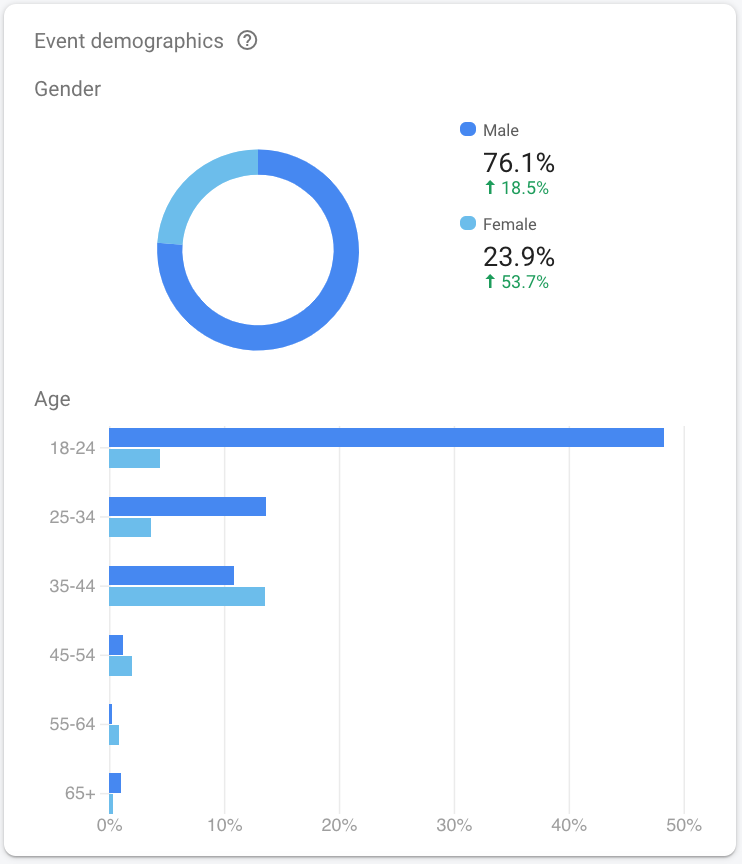
\includegraphics[width=8cm]{images/firebase/Firebase-event-demographics-pocketcode-android.png}
    \caption{Firebase Event Demographics for Pocket Code Android}
    \label{fig:Firebase-event-demographics-pocketcode-android}
\end{figure}

Practical options:
\begin{itemize}
    \item Do as others do?
    \item Proportionate exchange of value: users do not pay for the app, and few actively provide feedback. Organ donation is far more intrusive and yet English law is changing\footnote{\url{https://www.organdonation.nhs.uk/uk-laws/}} to presume consent~\cite{NHS_organ_donation_in_england} 
    \item Offer an opt-out
    \item Offer an opt-in
    \item leave the user to take action to provide information c.f. Kiwix-Android and Android Daisy Reader.
\end{itemize}

\subsection{Legal aspects of using mobile analytics for development and testing}

\begin{itemize}
    \item GDPR? The design and implementation of the mobile analytics may invoke GDPR considerations for whoever is responsible for the mobile app. In one of the appendices there is an example where concerns about the Firebase Android SDK and the dubious use of a \href{Firebase-SDK-ContentProvider}{ContentProvider}.
    \item PII vs non-PII information.
    \item \emph{``Who should make the online rules?"}~\citep{nytimes20210111_who_should_make_the_online_rules} Businesses in the USA have the right to make rules for what happens in their systems. Having basic rules, applied consistently, is vital in order for these businesses to operate effectively. However, the article notes \emph{``these companies’ rules are extensive, they are also capriciously applied and revised solely at their whim."}. The appeal processes and how they're enacted are seldom clear or effective. \textbf{MUST-DO} discuss legitimate developers ejected from Google Play Store~\citep{mark_dodson_medium_story, Martinez_2019}. %Plenty more material available from and via https://jilliancyork.com/
    \begin{itemize}
        \item \emph{``I can think all these tech companies made the right decision in the last few days but still feel extremely uncomfortable that they are in the position of acting as a Supreme Court — deciding for billions of people what is appropriate or legal expression and behavior."}
        \item \emph{``And while these companies’ rules are extensive, they are also capriciously applied and revised solely at their whim."}
        \item \emph{``Apple and Google are largely the only places for people to download smartphone apps. Amazon is one of a tiny number of companies that provide the backbone of many websites. Facebook, Google and Twitter are essential communications services for billions of people."}
    \end{itemize}
    Data is being bought and sold freely online~\citep{nytimes20210721_the_nightmare_of_our_snooping_phones} what's to stop the analytics data being sold. How would an app developer like their competitors buying and using their failure data? or a hacker who's looking to break into a mobile banking app? See also~\citep{nytimes20191221_total_surveillance_is_not_what_america_signed_up_for} and the series~\url{https://www.nytimes.com/interactive/2019/opinion/internet-privacy-project.html}. The Financial Times newspaper argues for a separation of roles of app store providers who are simultaneously the market owner and \emph{`` an app developer while operating as judge, jury, executioner and court of last appeal for all others."}. The article argues \emph{``If Apple [the subject in the article] does not itself update its App Store to distinguish between those roles and become more flexible and transparent, then it can hardly complain if legislators eventually deploy far more blunt instruments to enforce those changes."}~\citep{ft2020_apple_risks_losing_an_epic_challenge}.
    \item \emph{``According to noyb, the unique tracking code generated by each iPhone lets Apple and all iPhone app developers see how users behave without their knowledge or agreement"}~\citep{ft2020_apple_tracks_iphone_users_without_consent}.
\end{itemize}

Data ownership and safeguarding.

\subsection{Considerations and concerns when using Mobile Analytics}
\begin{itemize}
    \item Privacy:
    \item Costs: financial, data, privacy, performance, bloat:
    \item Who owns the data and who gets to use it?:
    \item Stewardship: Impact(s) of having access to sensitive and valuable data.
    \item Performance:
    \item Sufficiency: is the data we collect sufficient to enable us to achieve our objectives of improving testing.
    \item [Over] trust in decisions made by technology.
\end{itemize}


\subsection{"Data is the new gold"}

Sensitivity of allowing external access to analytics data, MUST-DO complete this section. 
% original text: "We can no longer provide this information outside of the company for sensitivity reasons ..."

\subsection{Human behaviours around automation}
% Confirmation bias (via Isabel)
The use of software automation can have deep implications on the humans involved, ranging from emotional stress and worries where testers on development teams can get stuck where tools are expected to solve problems (but don't)~\cite{evans2020stuck}, to potentially over-reliance on the decisions made by automation~\cite{cummings2004automation} and a complacency and bias in human interaction with automated and decision support systems~\cite{parasuraman_complacency_and_bias_in_human_use_of_automation}. 
My experiences of email discussions with the Google Engineering team provided an impression they over-believed in the correctness of their analytics tools and the inability of any outsider 
% Stress I'm considered an outsider even though I worked for Google.
being able to understand their system. This is somewhat ironic given that I was a senior software quality engineer at Google for four years and worked on assessing the behaviours and qualities of Google's mobile apps for several years during that role.

\section{Additional considerations}
This section covers several additional topics, including: abandoned apps, additional app stores beyond Google Play and beyond Android, and implications for apps stores for medical devices?

\subsection{Abandoned Apps}
Users are not the only people who many abandon apps, developers do so too. By the very nature of abandoning an app a developer is also likely to abandon the reports and data associated with that app, including data from mobile analytics. As many researchers discover there are many abandoned opensource source code repositories, and similarly various organisations, including AppBrain, have identified apps that are effectively abandoned. % MUST-DO add citation for AppBrain report.

\subsection{The Reaper Cometh}
AppBrain is a business that actively monitors and reports on Android Apps in the Google Play Store. The business was founded by two other ex-Google engineers. They state Google is actively culling Android apps from the Google Play store and estimate approximately 16\% of apps are \emph{"low quality apps"} and \emph{"unlikely to be useful"}~\footnote{\url{https://www.appbrain.com/stats/number-of-android-apps}} % Percentage of low quality apps: 16%


\subsection{Applicability to Other App Stores?}
App Stores were popularised for mobile apps for Android, iOS, and other smartphone platforms now extinct (\emph{e.g.} Windows Mobile), even if App Stores existed several years before smartphones did. % COULD_DO cite early versions of the Mobile Developer's Guide to the Galaxy, etc.

% Isabel: add a figure across the domains, inter-domain considerations. See her scanned notes.

They then spread to other mainstream operating systems including OSX, some Linux distributions, etc. using a similar business and software development model to the Android and iOS app stores. Recently, e.g. in 2019, App Stores were also reported for Radiology - for instance in an article in Harvard Business Review on \emph{What AI ``App Stores" will mean for Radiology}~\cite{hbr_what_ai_app_stores_mean_for_radiology}. The authors of the article envisage various benefits that emerge from applying a \emph{marketplace model} for these apps, including better feedback for developers. In tandem, the importance of incorporating appropriate analytics and ensuring they are trustworthy also seems worthy of further research and analysis. 

\section{Using Mobile Analytics as a fulcrum}
% Source a discussion with Joe Reeve on \nth{10} September 2021 where he proposed the idea of mobile analytics being used as a pivot point by teams to encourage, enable, and allow changes in behaviour without blaming the team. Here's this new source of data which can help us improve our app...
\begin{mdframed}

``On changing behaviour

The most valuable outcome of adopting a new tool is usually a change in business practices, rather than the tool itself.
Changing people’s behaviour is difficult, because it means implicitly telling them that the current behaviour is wrong. A new tool is a pivot point that acts as an excuse to change without having to acknowledge flaws.

There are various ways that adopting a tool impacts business practices, for enterprises this is typically the function of a product’s Customer Success team. I believe an important function of product design is to move as much education from Customer Success into the product. A great product should not only facilitate best practices, it should be a vector of change management to enforce them." Joseph E. Reeve, \nth{10} September 2021 in discussion.
\end{mdframed}

\section{Left untended, entropy returns}
Several of the projects described in the case studies have had increased failure rates post the case studies, as confirmed by reviewing the relevant analytics reports which continued to be made available for research purposes. In each case, the increase occurred after a loss in focus on actively addressing causes of production errors being reported by the respective analytics tools.

\textbf{Post case study - Kiwix Android}
The Kiwix Android case study was scaled back in early 2020, however I continued to monitor it as a background activity with the agreement of the project leads. One of the many side-effects of the Covid-19 pandemic was a significant reduction in funding for the Kiwix project in Summer 2020 which culminated in the end of the funded lead-developer role for the Android codebase. The lead developer finished working on the project in late 2020 and since then the project has been mainly maintained by a mix of volunteers on a part-time basis. 

The crash and ANR rates have both increased in 2021, and are 0.73\% and 0.46\% respectively for the 30 days to \nth{11} June 2021 for the Kiwix Android app (the most recent release is v3.4.4 released on \nth{20} May 2021). Many of the most common crashes are related to the embedded WebView component... TBC



\section{Summary of the Discussion Chapter}
My research indicates mobile analytics can be used to effectively and efficiently improve the measured stability qualities of various Android apps from disparate sources, development teams and software stacks. And yet, there are appear to be material flaws in key analytics tools. My research touches on various implications of using analytics including which projects are best served by the integral analytics Google provides in Google Play Console. There are numerous areas of potential interest to researchers and industry alike including the integrity and accuracy of the various tools and reports. I will introduce my planned future work in the Future Work chapter.


Much remains to do in the area of applying mobile analytics to the development practices. Real-world bugs, including several I experienced recently and described next are not likely to be detected by the developers without a combination of some of all of: improved testing practices, rich in-app feedback, and using and applying in-app mobile analytics.

A couple of examples of poor user experiences that don't involve crashes or freezes (so would not be detected using the platform-level analytics) are, the Financial Times Android app: Figure~\ref{fig:ft_android_app_bsod}, and The Times newspaper iOS app: ``Cannot find article: Apologies, this article no longer exists." Figure~\ref{fig:thetimes-ios-this-article-no-longer-exists}. Of these, the missing article could be recorded easily using in-app error reporting (it might be detected by a non-fatal exception using a crash-reporting library or mobile analytics). The black screen is likely to be harder to report on (as if the developers were aware of the potential for the problem they could add error-handling and error-recovery logic).

\begin{figure}[!htbp]
    \centering
    \subfloat[What the user sees] {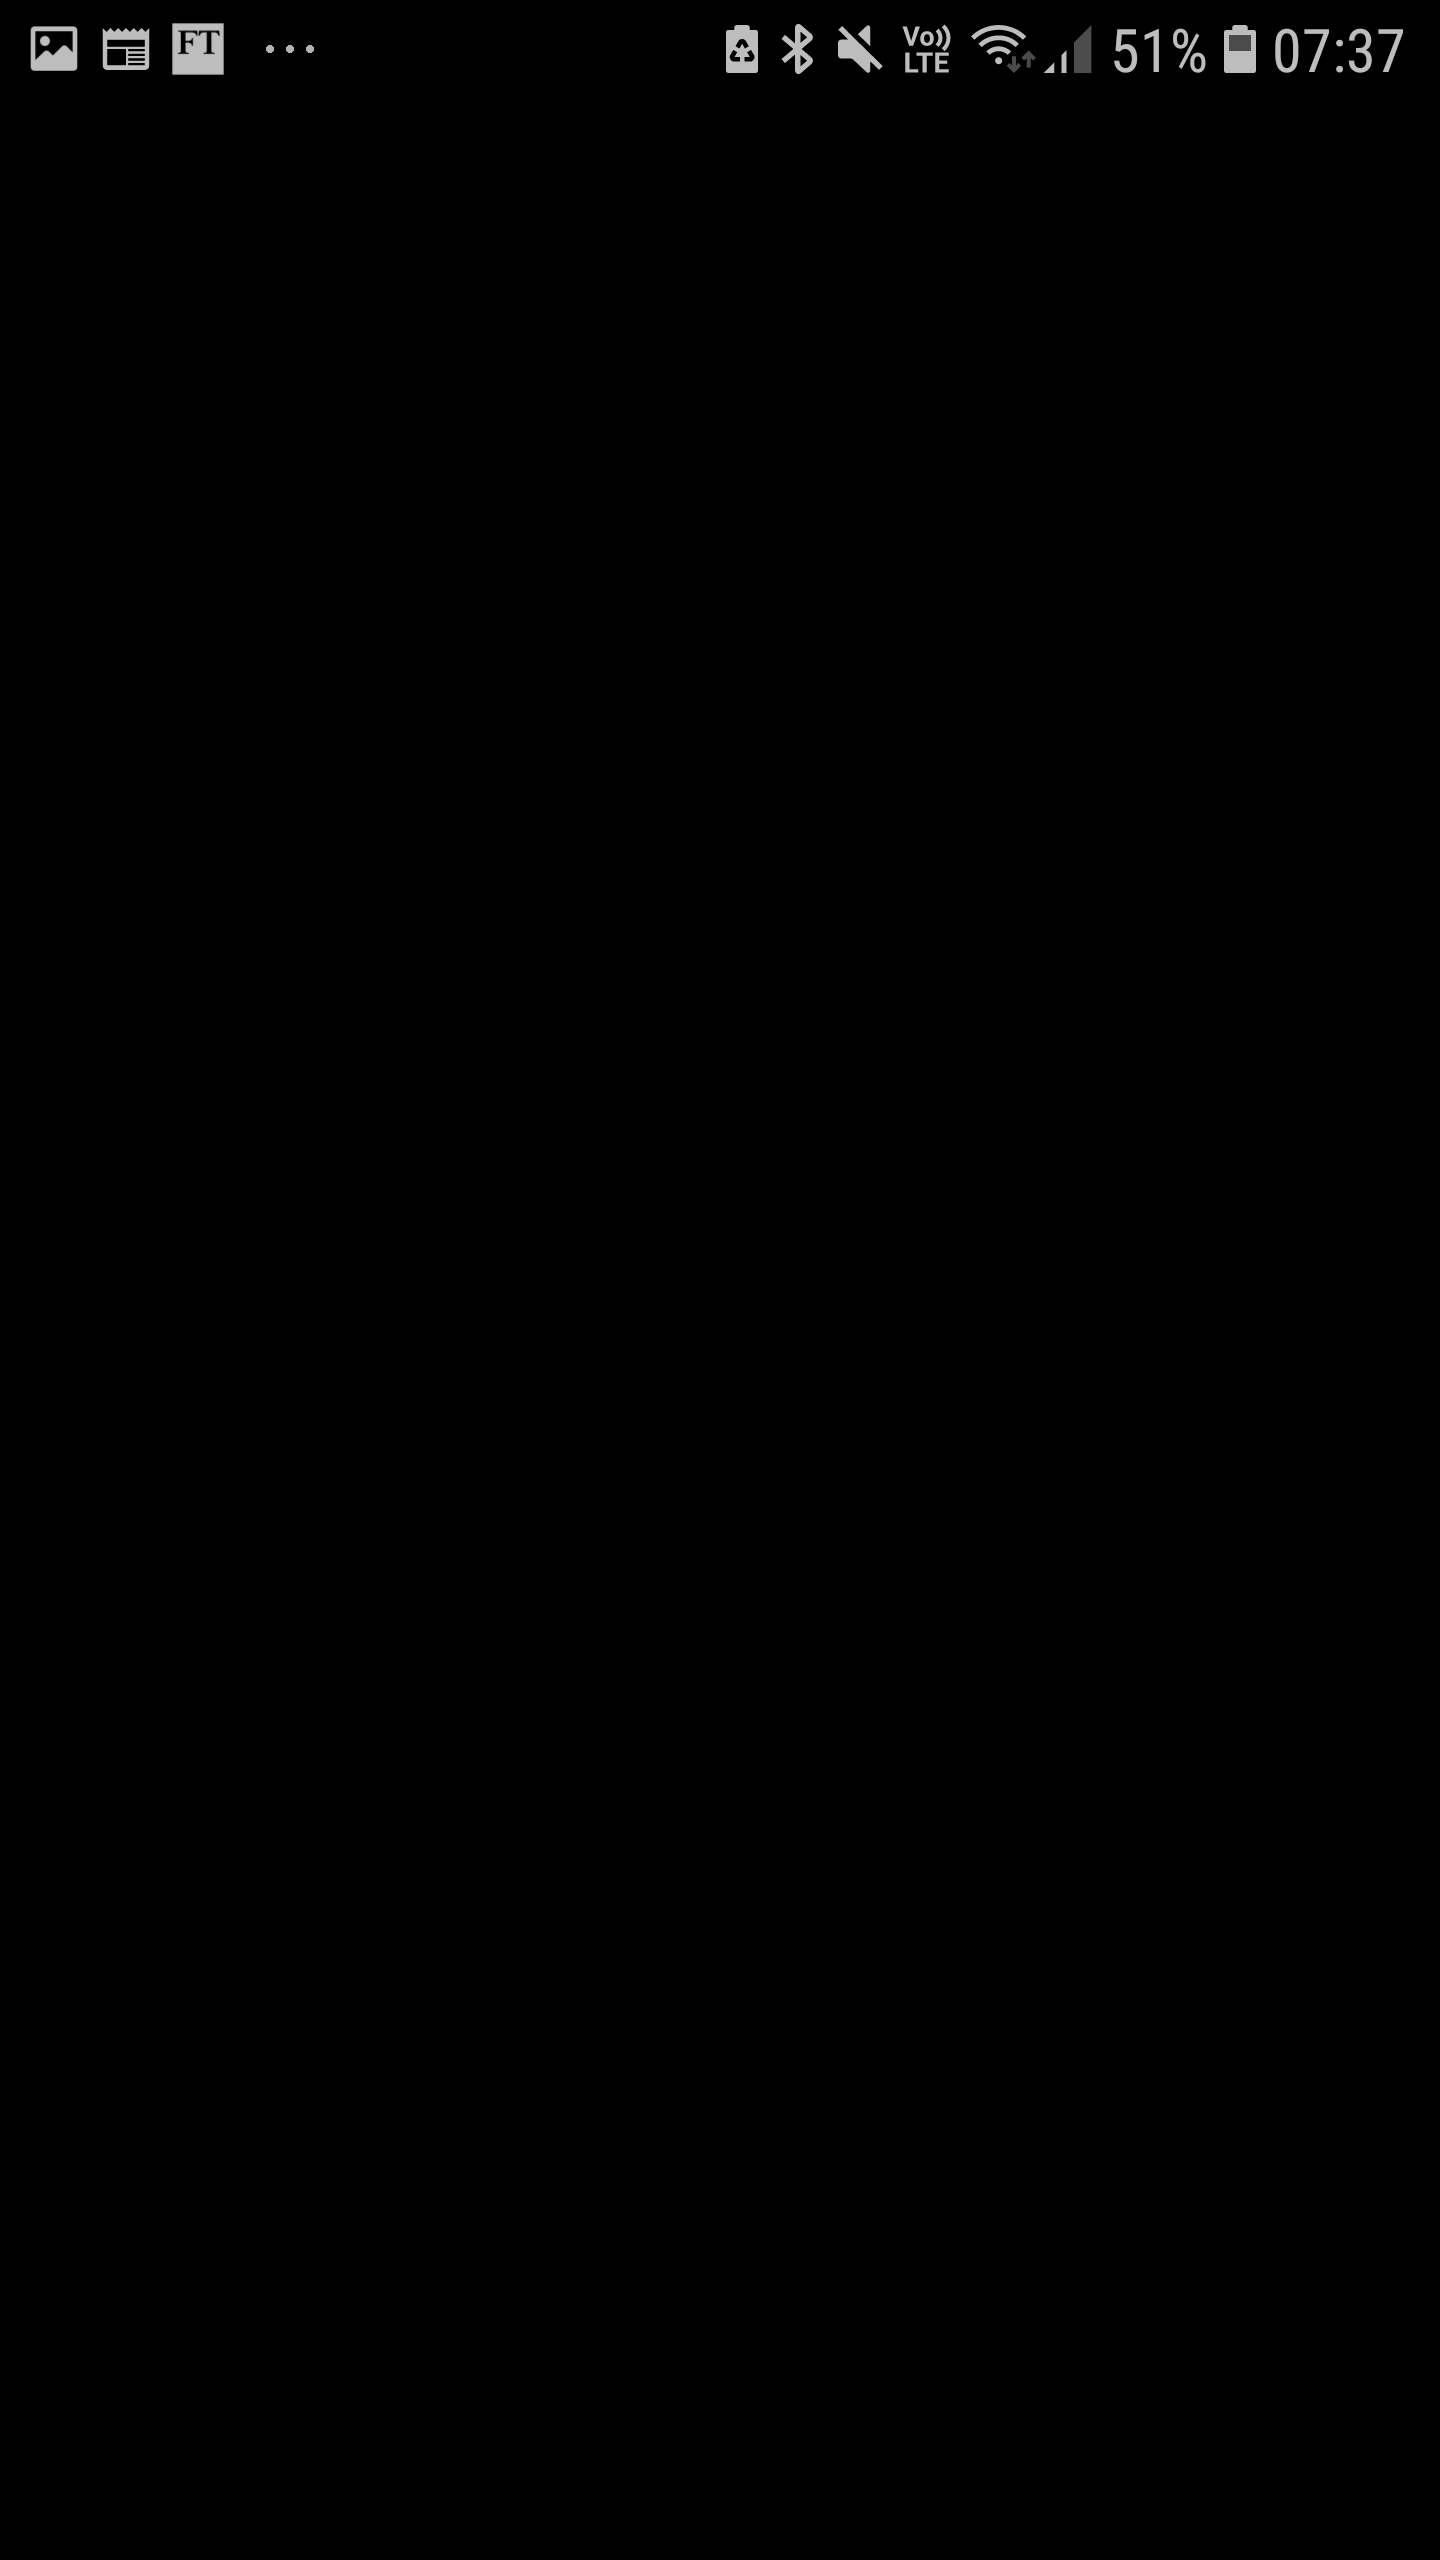
\includegraphics[width=0.45\textwidth]{images/android-screenshots/Screenshot_20200928-073727_FT.jpg}\label{fig:android_ft_GUI}}
    \hfill
    \subfloat[The FT app in the task list] {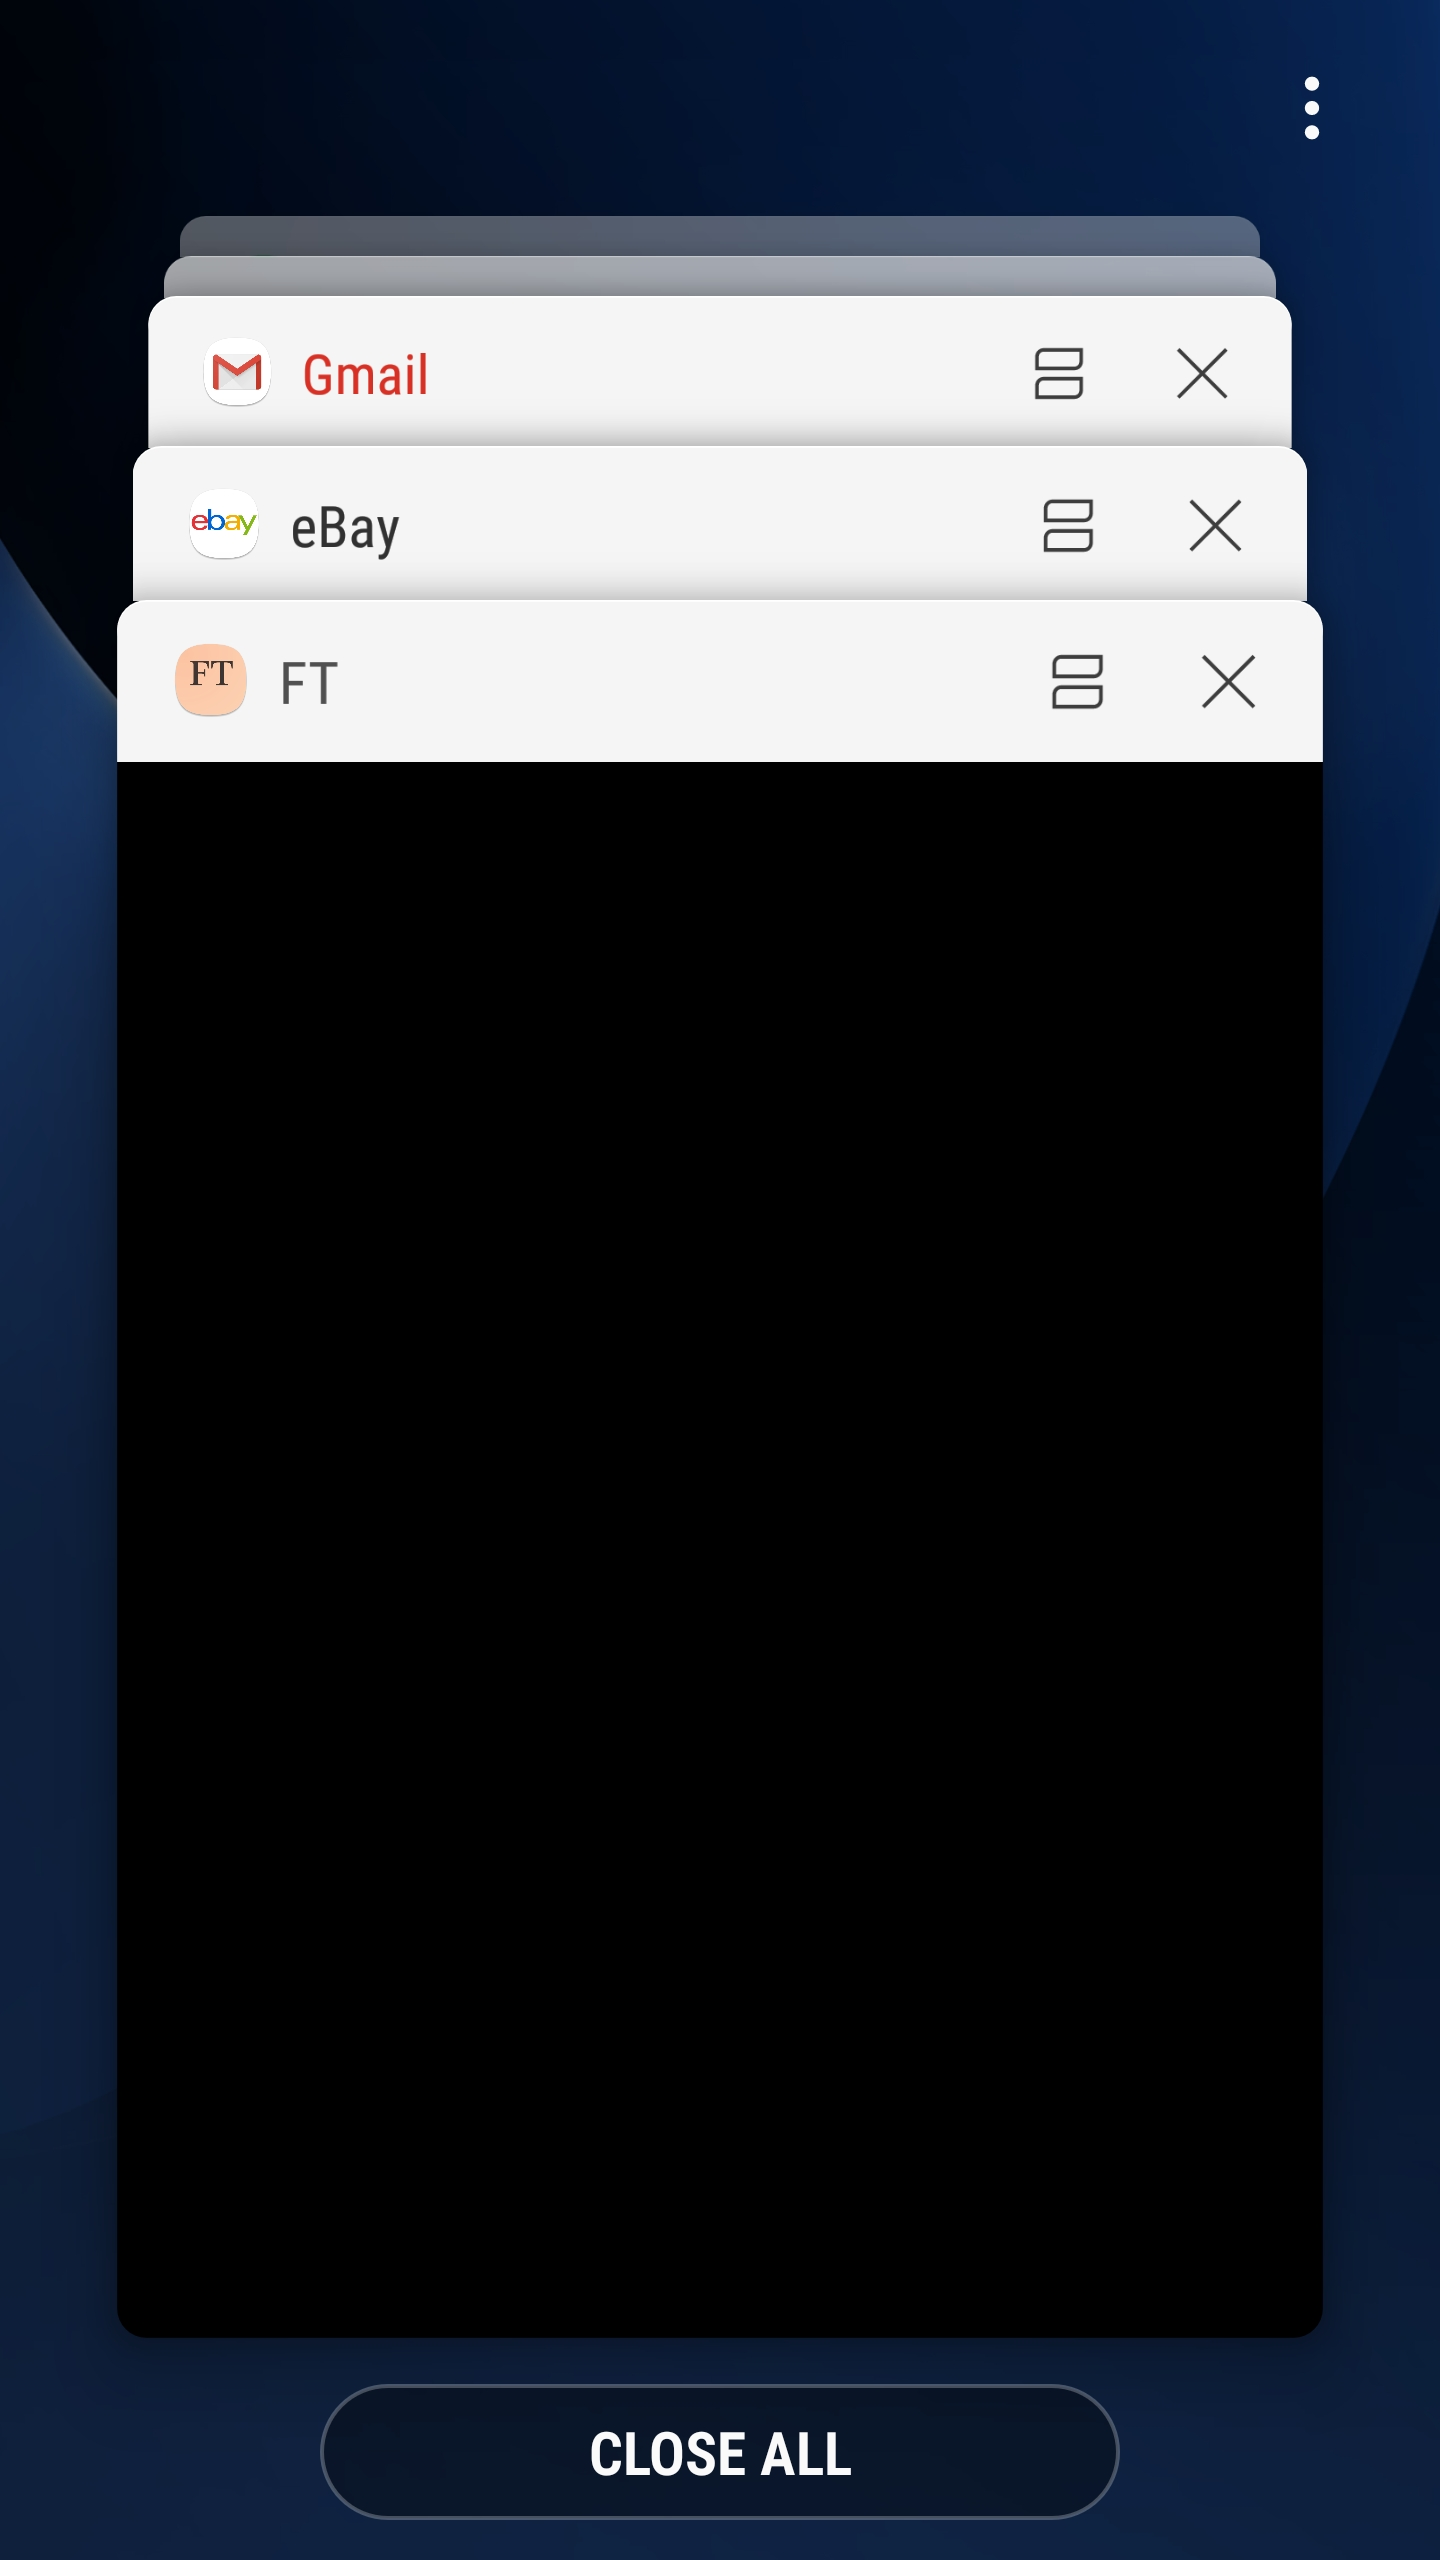
\includegraphics[width=0.45\textwidth]{images/android-screenshots/Screenshot_20200928-073745_FT.jpg}\label{fig:ft_android_app_in_task_list}}
      \caption{Black screen when notification selected}
    \label{fig:ft_android_app_bsod}
\end{figure}

\begin{figure}[!htbp]
    \centering
    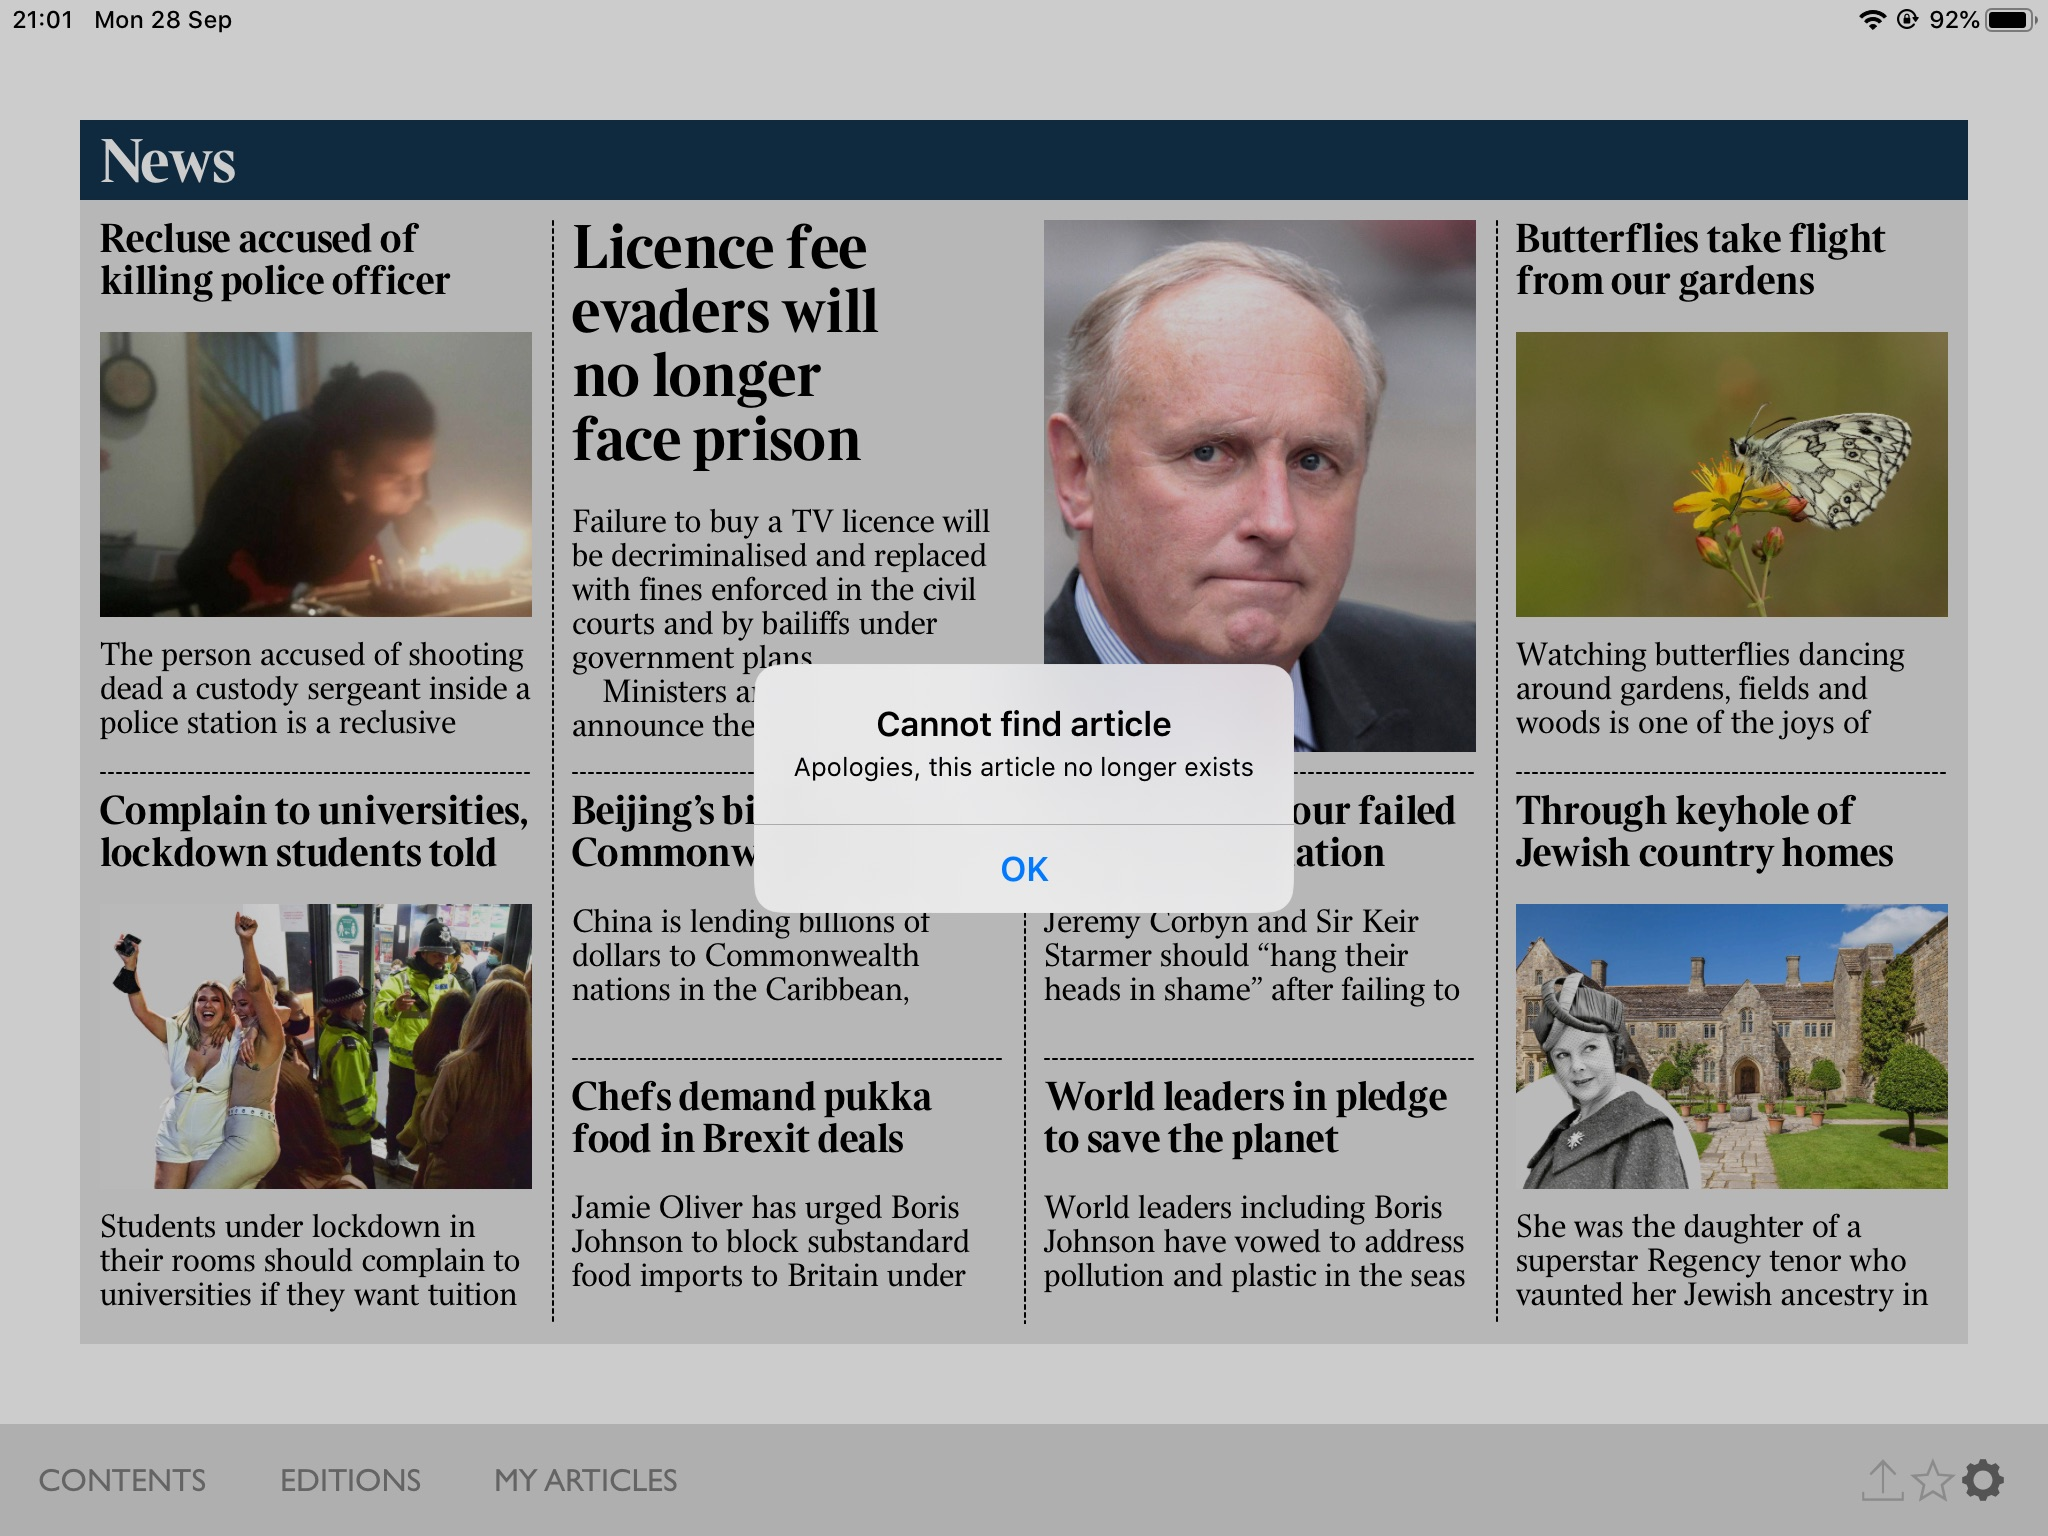
\includegraphics[width=13cm]{images/ios-screenshots/The-Times-iOS-Screenshot-2020-09-28.png}
    \caption{The Times iOS app: ``this article no longer exists" \nth{28} September 2020.}
    \label{fig:thetimes-ios-this-article-no-longer-exists}
\end{figure}
